\section{Datos a analizar}

\textbf{AVISO:} Debido a que el workflow ejecutado ocupa demasiado espacio adjuntaré en PRADO solo el workflow sin ejecutar, aunque como se ve en las capturas de esta memoria se ha conseguido ejecutar sin problemas y obtener los resultados finales para realizar la práctica.

Los datos a analizar se tratan de opiniones sobre películas de la base de datos IMDb. La información de la que disponemos es de un identificador, la URL de la opinión, el texto que conforma la opinión e información sobre si la opinión es positiva o negativa.

En nuestro caso utilizaremos el texto como documento y el identificador para realizar operaciones sobre los datos y mantener la coherencia al realizar algunas operaciones sobre los datos.

\section{Lectura de los datos}

Para la lectura de los datos simplemente leemos el fichero CSV con la información, transformamos la columna de la review de string a documento, y finalmente nos quedamos con la columna de indice, documento y el sentimiento asociado. Esta salida será la que utilizaremos para clasificar los documentos tanto utilizando diccionarios como modelos de clasificación, aunque para utilizarlos en modelos de clasificación primero necesitaremos preprocesarlos.

\section{Preprocesamiento para clasificación}

Para utilizar modelos de clasificación primero se ha aplicado el siguiente preprocesamiento a los documentos:

\begin{figure}[H]
	\centering
	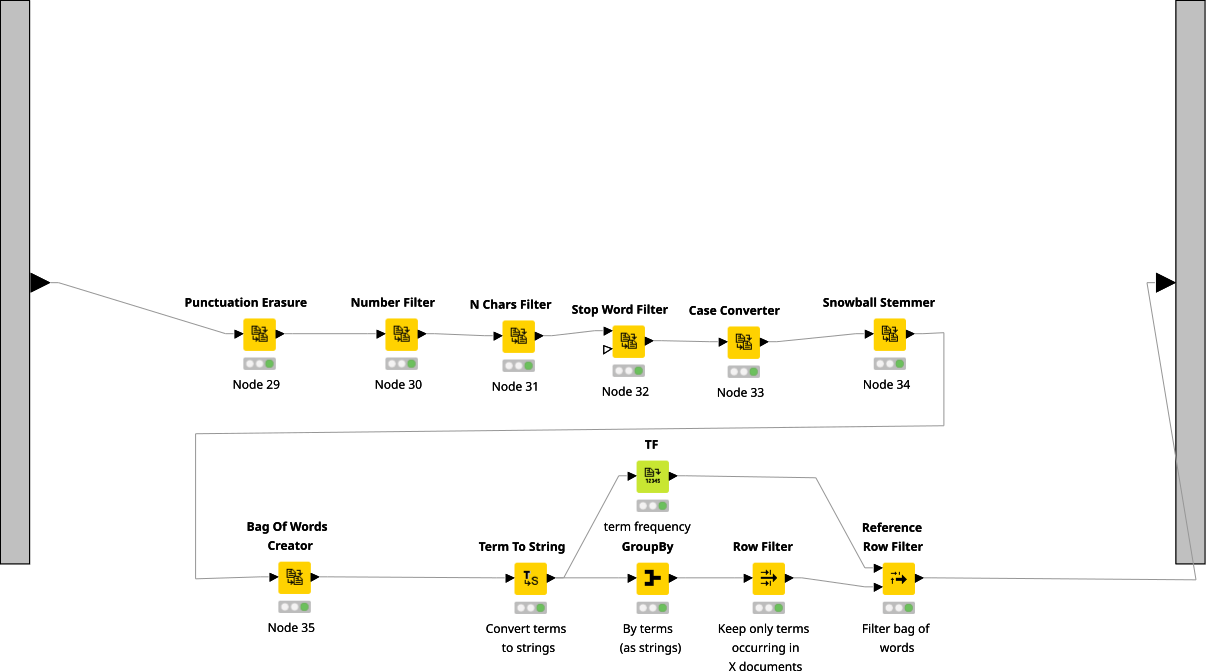
\includegraphics[width = \textwidth]{preprocesamiento.png}
	\caption{Preprocesamiento aplicado a los documentos para modelos de clasificación.}
	\label{fig:preprocesamiento}
\end{figure}


Como vemos, simplemente limpiamos los documentos de caracteres especiales, palabras muy cortas, y pasamos todas las palabras a minusculas. Tras esto nos quedamos con los términos más frecuentes, que será con los que trabajemos.

\section{Uso de métodos de clasificación}

Una vez realizado el preprocesamiento simplemente separamos los documentos en entrenamiento y test, y aplicamos los métodos de clasificación.

En mi caso he escogido utilizar los clasificadores Random Forest y Logistic Regression:

\begin{figure}[H]
	\centering
	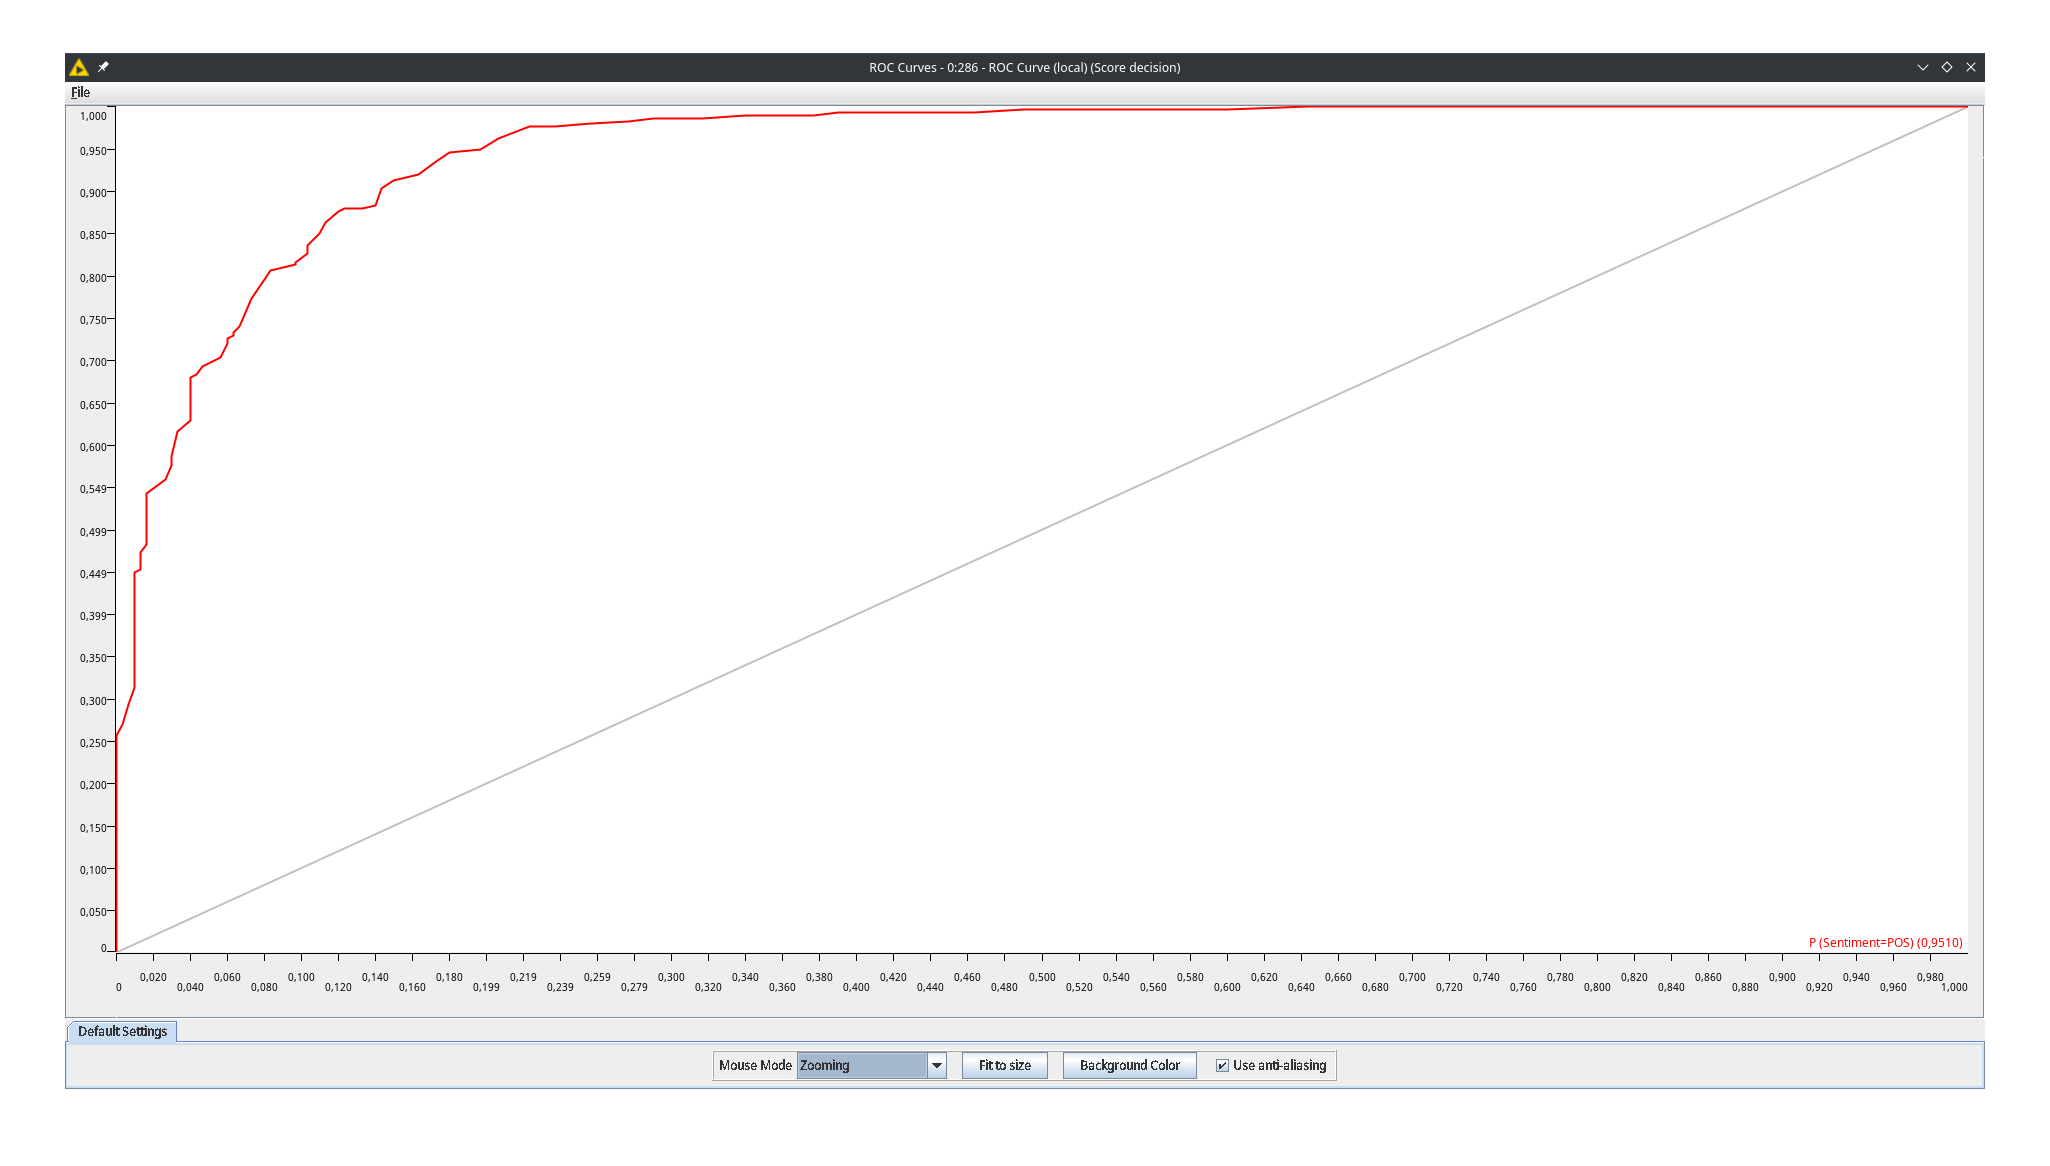
\includegraphics[width = \textwidth]{roc_RF.png}
	\caption{Curva ROC obtenida del modelo Random Forest.}
	\label{fig:roc_RF}
\end{figure}

\begin{figure}[H]
	\centering
	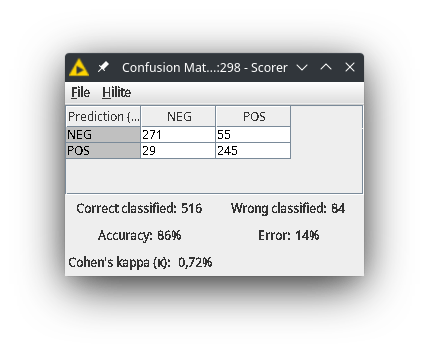
\includegraphics[scale = 0.6]{matriz_RF.png}
	\caption{Matriz de confusión obtenida del modelo Random Forest.}
	\label{fig:matriz_RF}
\end{figure}

\begin{figure}[H]
	\centering
	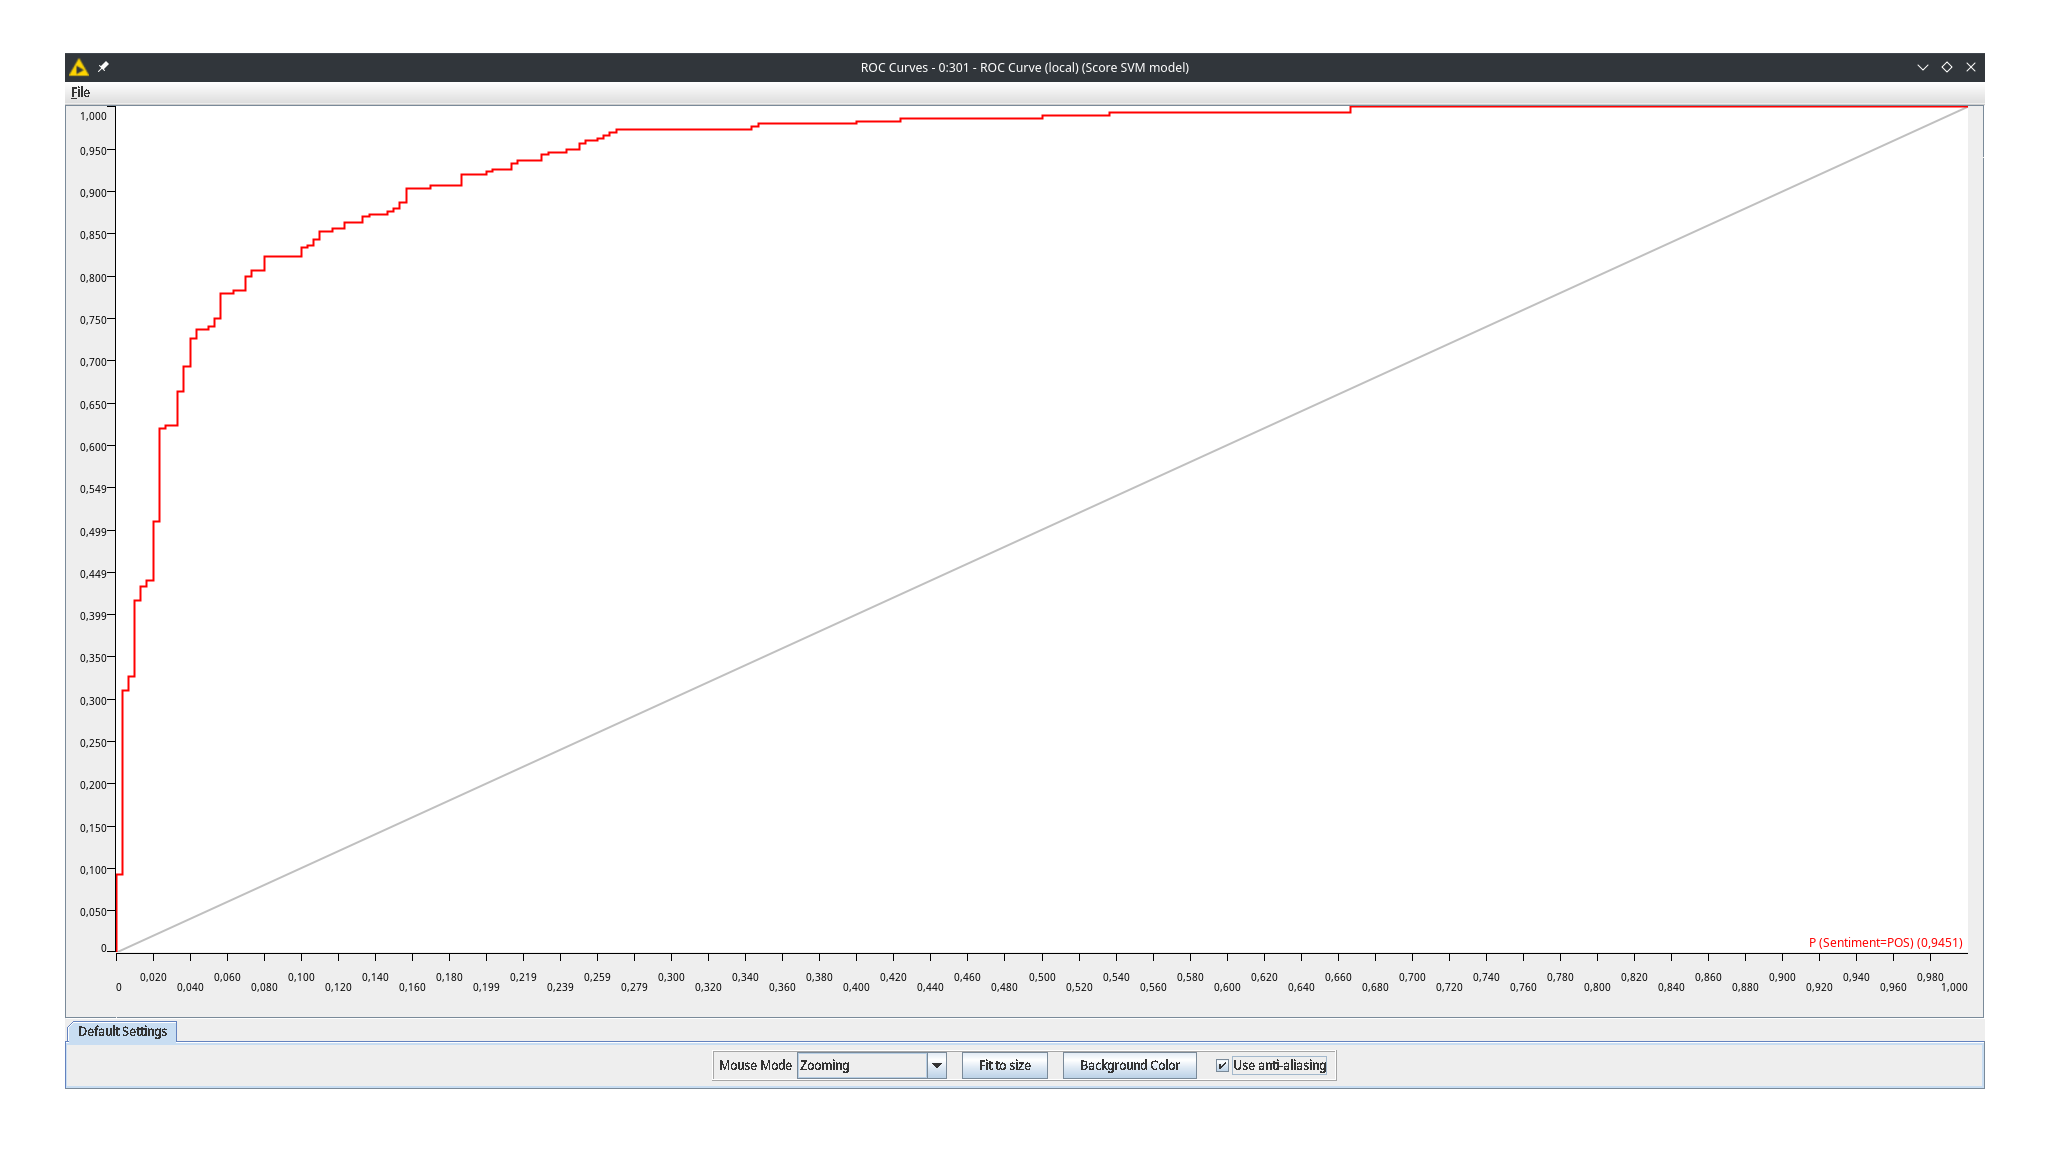
\includegraphics[width = \textwidth]{roc_LR.png}
	\caption{Curva ROC obtenida del modelo Logistic Regression.}
	\label{fig:roc_LR}
\end{figure}

\begin{figure}[H]
	\centering
	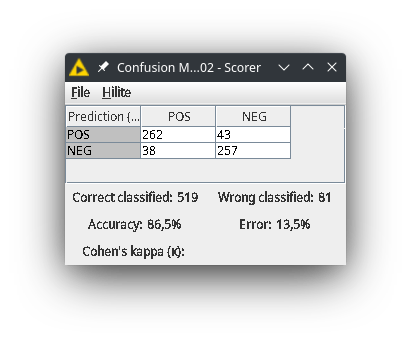
\includegraphics[scale = 0.6]{matriz_LR.png}
	\caption{Matriz de confusión obtenida del modelo Logistic Regression.}
	\label{fig:matriz_RL}
\end{figure}

Como vemos, con ambos modelos conseguimos resultados similares, alrededor del 85-90\% de acierto, una tasa de acierto bastante buena. Vamos comparar estos resultados con utilizar diccionarios.


\section{Uso de diccionarios para análisis de sentimientos}

El uso de diccionarios para predecir opiniones se basa en, a cada palabra, asociar una opinión positiva o negativa, y contar si en un documentos existen más palabras positivas o negativas.

Para comenzar, la primera tarea es leer dichos diccionarios.

\subsection{Lectura de diccionarios}

Debido a que cada diccionario tiene un formato un poco distinto, cada nodo de lectura es un poco distinto, lo único en lo que coinciden es que todos sacan en la primera salida las palabras positivas, y en la segunda las palabras negativas:

\begin{figure}[H]
	\centering
	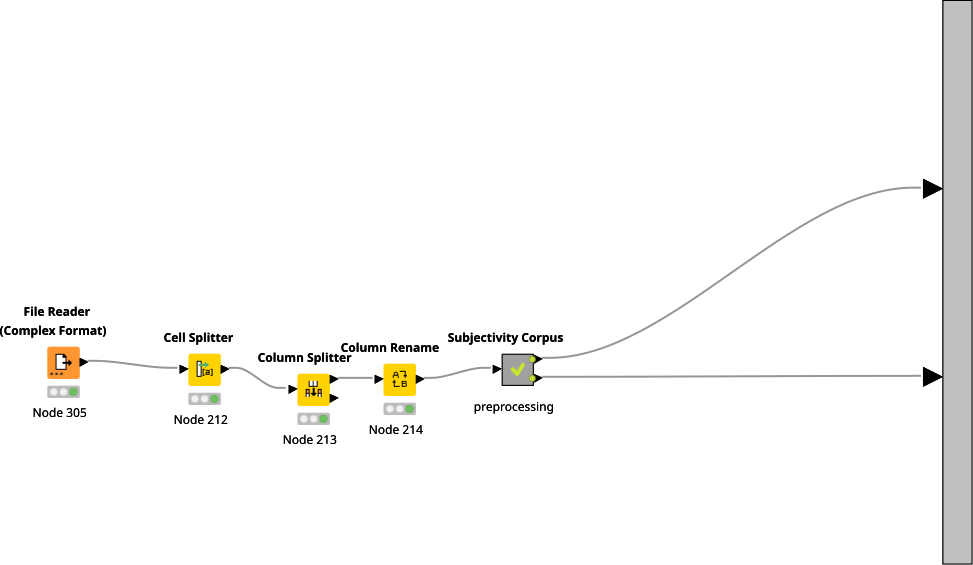
\includegraphics[width = \textwidth]{leer_subjectivity.png}
	\caption{Workflow de lectura del diccionario Subjectivity.}
	\label{fig:leer_subjectivity}
\end{figure}

La lectura de este diccionario ya la hicimos en clase. Se trata de leer el fichero, y usando expresiones regulares quedarnos únicamente con los términos y el sentimiento asociado. Una vez tenemos eso, filtrar dependiendo del sentimiento para separar en positivos y negativos.

\begin{figure}[H]
	\centering
	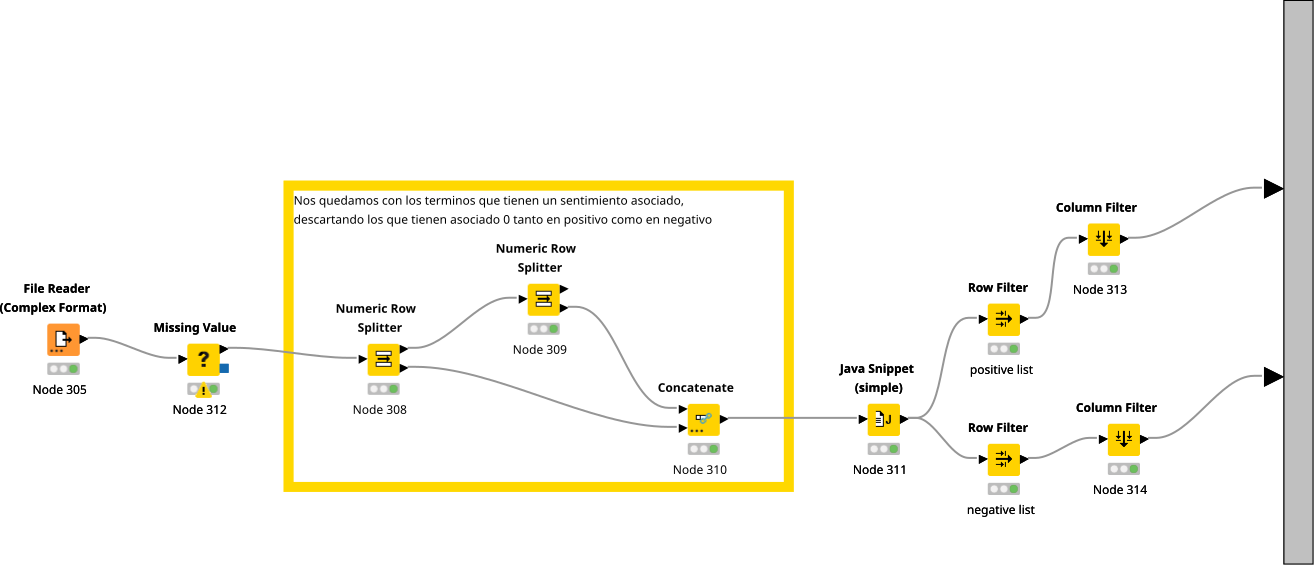
\includegraphics[width = \textwidth]{leer_sentiwordnet.png}
	\caption{Workflow de lectura del diccionario SentiWordNet.}
	\label{fig:leer_sentiwordnet}
\end{figure}

En SentiWordNet las palabras no tienen asociado un sentimiento, si no un valor de pertenencia a sentimiento positivo y sentimiento negativo. Por este motivo, la lectura no es tan simple como leerlos y escoger si una palabra es positiva o negativa. Lo primero que realizamos es limpiar todas las palabras que no tienen un sentimiento asociado (tienen un 0 en pertenencia a sentimiento positivo y 0 en pertenencia a sentimiento negativo). Tras esto, usando un Java Snippet, generamos una nueva columna que decide si una palabra es positiva o negativa, dependiendo si el nivel de pertenencia a un sentimiento positivo es mayor al nivel de pertenencia a un sentimiento negativo, o por el contrario es negativa. Tras esto ya tenemos el sentimiento asociado, lo dividimos y será el resultado de la lectura.

\begin{figure}[H]
	\centering
	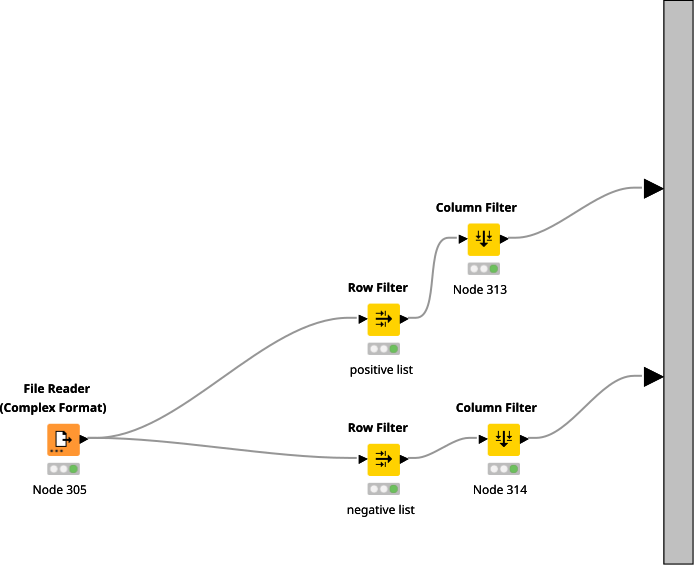
\includegraphics[width = \textwidth]{leer_senticnet.png}
	\caption{Workflow de lectura del diccionario SenticNet.}
	\label{fig:leer_senticnet}
\end{figure}

En este caso la lectura es muy simple, ya que existe una columna si nos dice si una palabra es positiva o negativa.

\subsection{Uso para decidir el sentimiento de documentos}

Debido a que se ha estandarizado la salida de los diccionarios (devuelve una tabla con las palabras positivas y otra con las palabras negativas), se ha podido realizar un único workflow que recibe tres entradas, los documentos, las palabras positivas y las negativas, para trabajar independientemente del diccionario.

\begin{figure}[H]
	\centering
	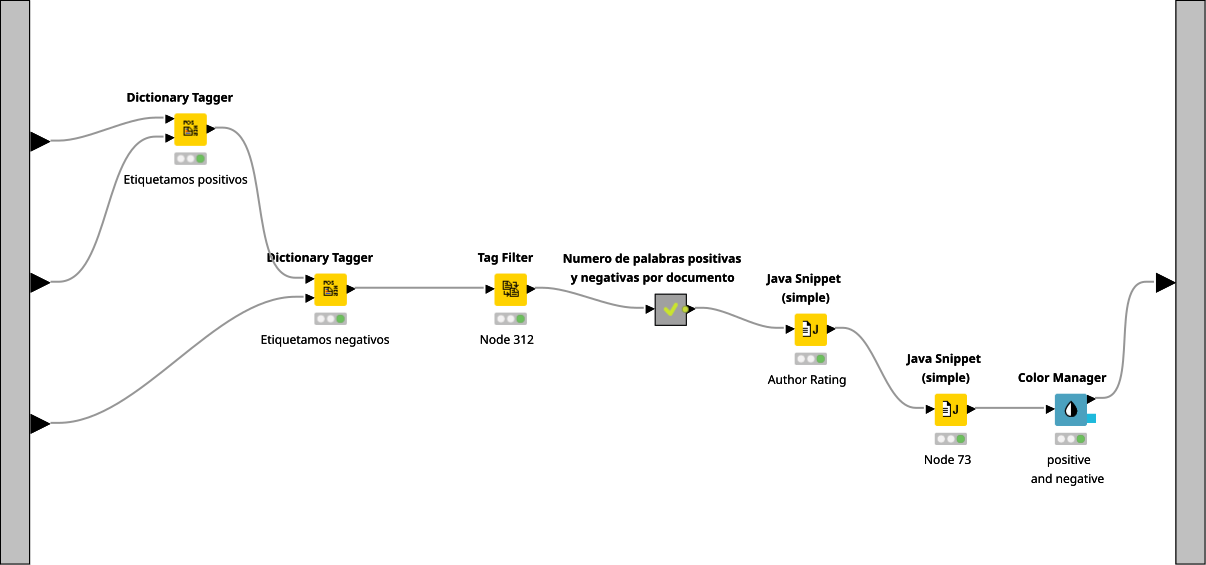
\includegraphics[width = \textwidth]{clasificar_diccionarios.png}
	\caption{Workflow de clasificación usando un diccionario.}
	\label{fig:clasificar_diccionarios}
\end{figure}

Como vemos, primero se usa un Dictionary Tagger para etiquetar las palabras positivas de los documentos, luego otro para las palabras negativas, filtramos por las palabras que tienen asociada una etiqueta de sentimiento, y tras esto simplemente hacemos un conteo para ver si en un documento existen más palabras positivas o negativas. Con esto ya tendríamos una clasificación de cada documento, dependiendo de si hay un mayor número de etiquetas positivas o negativas.

Los resultados obtenidos son los siguientes:

\begin{figure}[H]
	\centering
	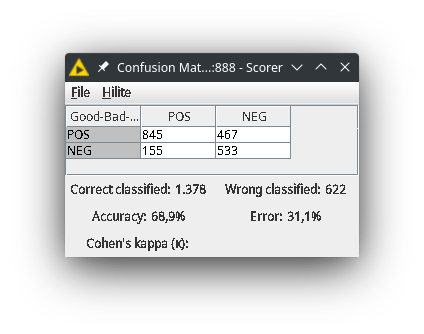
\includegraphics[scale = 0.6]{matriz_subjectivity.png}
	\caption{Matriz de confusión obtenida del diccionario Subjectivity.}
	\label{fig:matriz_subjectivity}
\end{figure}

Usando Subjectivity obtenemos unos resultados por debajo del 70\% de tasa de acierto, fallando especialmente en los falsos positivos.

\begin{figure}[H]
	\centering
	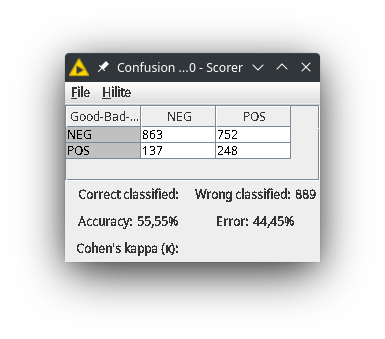
\includegraphics[scale = 0.6]{matriz_sentiwordnet.png}
	\caption{Matriz de confusión obtenida del diccionario SentiWordNet.}
	\label{fig:matriz_sentiwordnet}
\end{figure}

Los resultados de SentiWordNet son aún peores, con una tasa de acierto del 55\%, aunque como vemos el número de falsos negativos sigo igual, solo hemos empeorado el problema que ya se tenía con los falsos positivos.

\begin{figure}[H]
	\centering
	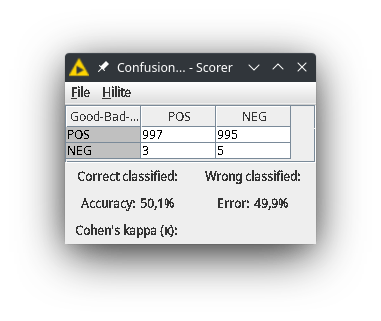
\includegraphics[scale = 0.6]{matriz_senticnet.png}
	\caption{Matriz de confusión obtenida del diccionario SenticNet.}
	\label{fig:matriz_senticnet}
\end{figure}

SenticNet se comporta mucho peor, clasificando todos los documentos como positivos, por lo que los resultados son como tirar una moneda al aire, con una tasa de acierto del 50\%.

\section{Comparación entre uso de modelos de clasificación y de diccionarios}

Como hemos visto en el apartado anterior, los modelos de clasificación son muy superiores al uso de diccionarios. Se puede intuir a que el uso de diccionarios se limita a hacer un conteo de palabras, sin tener en cuenta el contexto ni que combinaciones de palabras aparecen juntas en los documentos, mientras que en un modelo de clasificación esto si se puede tener en cuenta.

Con modelos simples hemos obtenidos muy buenos resultados, así que cabría esperar que si además utilizásemos modelos de redes neuronales recurrentes, las cuales son capaces de recordar el contexto, como modelos especializados en NLP como BERT, los resultados serían todavía mejores, por lo que el uso de diccionarios no sería de tanto interés en este problema.

\section{Workflow final}


El flujo final realizado a lo largo de la práctica es el siguiente:

\begin{figure}[H]
	\centering
	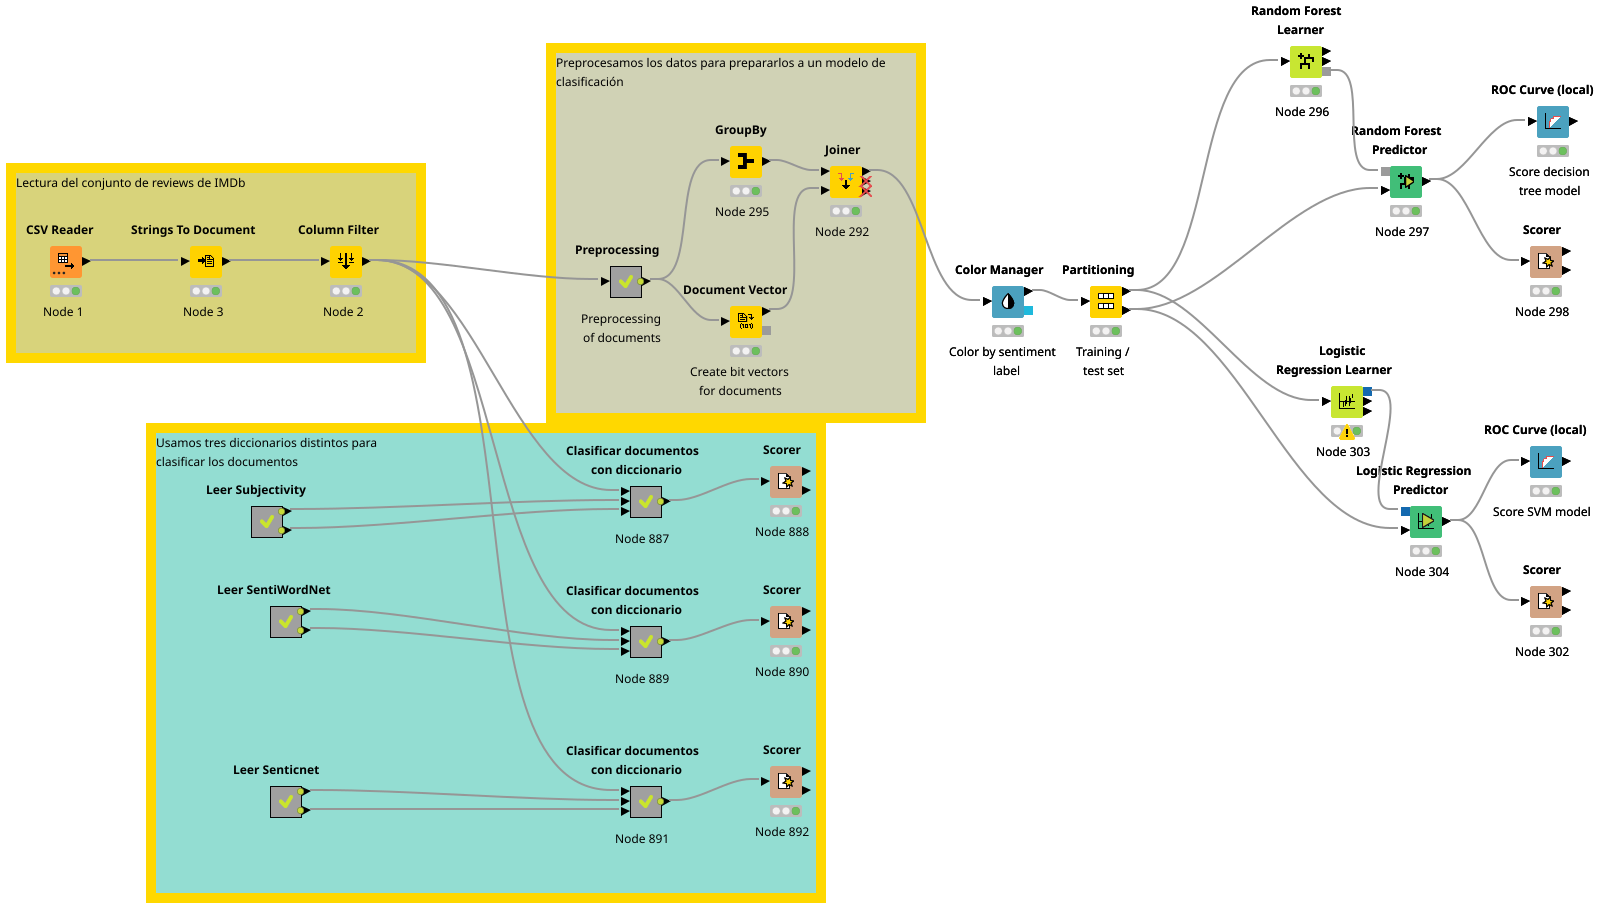
\includegraphics[width = \textwidth]{workflow_knime.png}
	\caption{Workflow final de KNIME.}
	\label{fig:workflow_knime}
\end{figure}


Gracias a la lectura unificada de documentos, y un preprocesado común, se ha conseguido un workflow bastante simple, del que se han podido reutilizar muchas partes, además de obtener unos buenos resultados cuando se utilizaban modelos de clasificación.
